\chapter{Introduction to Software Engineering and LLMSE}

recupera fino a pagine 54


\section{The agile manifesto}


\begin{enumerate}
  \item Our highest priority is to satisfy the customer through early and
        continuous delivery of valuable software
  \item Welcome changing requirements, even late in development. Agile
        processes harness change for the customer's competitive advantage.
  \item Deliver working software frequently, from a couple of weeks to a
        couple of months, with a preference to the shorter timescale.
  \item Business people and developers must work together daily
        throughout the project.
  \item Build projects around motivated individuals. Give them the environment
        and support they need and trust them to get the job done.
  \item The most efficient and effective method of conveying information to and
        within a development team is face-to-face conversation.
  \item Working software is the primary measure of progress.
  \item Agile processes promote sustainable development. The sponsors,
        developers, and users should be able to maintain a constant pace
        indefinitely.

  \item Continuous attention to technical excellence and good design
        enhances agility.
  \item Simplicity - the art of maximizing the amount of work not done- is
        essential.
  \item The best architectures, requirements, and designs emerge from
        self-organizing teams.
  \item At regular intervals, the team reflects on how to become more
        effective, then tunes and adjusts its behavior accordingly.
\end{enumerate}

\subsection{From manifesto to practice}
Tight collaboration between developers and stakeholder over the
entire course of the project.

Self-organizing teams

Software SCRUM is the most used methodology

Other methodologies like Kanban and eXtreme Programming are
less used


\section{SCRUM}


\begin{flushleft}
  \begin{minipage}{0.65\linewidth}

    Evolution of the iterative software model.
    Produt owner: the guy who we need to satisfy. It produce a product backlog (what a user wants),
    a list of features that we need to implement. This is the thruth.

    The scrum master acts as a coach with a business or pshychology background.


  \end{minipage}%
  \hfill
  \begin{minipage}{0.3\linewidth}
    \centering
    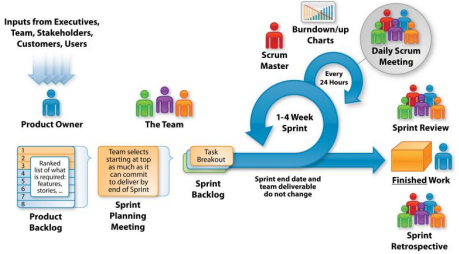
\includegraphics[width=1\linewidth]{content/Parts/images/2026-11-09-09-06-19.png}
  \end{minipage}
\end{flushleft}

\subsection{What makes a good PBI: INVEST}


\begin{itemize}
  \item Independent
  \item Negotiable
  \item Valuable
  \item Estimable
  \item Small
  \item Testable
\end{itemize}

\section{LLM4SE}

\subsection{Definitions}

\subsubsection{AI4SE} Applies augmented intelligence and machine learning
techniques to support systems engineering practicesMore and more
systems are software controlled.

\subsubsection{SE4AI} Applies systems engineering methods to learning- based
systems' design and operation

\subsubsection{LLM-Based Software Engineering (LLMSE)}
Integration of Large Language Models (LLMs) into software engineering.
It encompasses any application where the products or processes leverage LLMs to
enhance development and operational efficiency.

\subsubsection{LLM Application}
Defined as any task or activity that benefits from
LLM insights. This broad definition captures the essence of LLM's
versatility across various domains, offering improvements through its
advanced computational capabilities.

\subsubsection{LLM Consumer}
Any individual, system, or process that utilizes LLM
outputs. This definition acknowledges the wide array of LLM
beneficiaries, from developers and businesses to automated systems,
all relying on LLM-generated intelligence

\subsubsection{Assured LLMSE}
This innovative approach guarantees the reliability of
LLM outputs. Every response from an LLM, possibly after undergoing
post-processing, comes with a verifiable assertion of its usefulness.
Assured LLMSE sets a standard for trust and quality in the application
of LLMs in software engineering

\section{Criteria for LLM selection}
The selection of LLM for SE tasks should involve more careful consideration
rather than arbitrary choice.

Key factors guiding this selection are:

\begin{itemize}
  \item  Model proficiency in understanding the context of the code
  \item Ability to generate relevant content
  \item  Responsiveness to fine-tuning
  \item  Demonstrated performance in SE-specific benchmarks
\end{itemize}


\subsection{Task-specific fine tuning}
A notable trend is the customization of LLMs for precise SE tasks.
By fine tuning models with datasets tailored to specific functions (e.g., bug
detection or code review) researchers are able to achieve marked
performance improvements.


\subsection{Sources for datasets}

Data determines the generalization ability, effectiveness, and performance of the
models.

Four different methods can be used for data collection:

\begin{itemize}
  \item \textbf{Open-source datasets}: publicly accessible collections of data that are often disseminated
        through open-source platforms or repositories
  \item \textbf{Collected datasets}: datasets compiled from the researchers directly from a multitude of
        sources, including (but not limited to) major websites, forums, blogs, and social media
        platforms.
  \item \textbf{Constructed datasets}: specialized datasets that researchers create by modifying or
        augmenting collected datasets to better align with their specific research objectives.
  \item \textbf{Industrial datasets}: obtained from commercial or industrial entities; often contain
        proprietary business data, user behaviour logs, and other sensitive information.
\end{itemize}


\section{Types of data used in LLM4SE}
\begin{itemize}
  \item Text-based datasets: datasets composed by textual (natural language)
        elements, or non-functioning code (snippets).

  \item Code-based datasets: datasets composed only by code artefacts.


  \item Graph-based datasets: can be used when representing the GUI states of an
        application to develop or test.

  \item Software repository based-datasets: compilations of data extracted from
        version control systems, such as Git repositories, containing code,
        documentation, and related artefacts.

  \item Combined datasets: combinations of multiple types of datasets.
\end{itemize}


\section{Prompt Engineering}

We selected the LLMs then we selected the datasets and now we need to select the prompts.

The full chain is:

\begin{enumerate}
  \item Architecture
  \item Select LLM
  \item Select datasets
  \item Select prompts
  \item Evaluate
\end{enumerate}



